\subsection{MPC Controllers}
\label{subsec:mpc_controllers}

Model Predictive Control (MPC) is an advanced control strategy widely used in industrial and engineering applications. It involves an optimization procedure which is continuously reinitialized as time goes on. This continuous adaptation of the control strategy makes the model very flexible and efficient in various applications.

There exist many versions of MPC but, given the limited computational resources available, we have chosen to implement the linear MPC with constraints on the output variable. This version of MPC is based on a linear model of the system and is computationally less expensive than the nonlinear version.

The system is typically represented in discrete time as:

\begin{equation}
    \begin{aligned}
        \mathbf{x}_{k+1}=\mathbf{A}\mathbf{x}_{k}+\mathbf{B}\mathbf{u}_{k} \\
        \mathbf{y}_{k}=\mathbf{C}\mathbf{x}_{k}
    \end{aligned}
\end{equation}

where $x_k$ is the state vector at time $k$, $\mathbf{u}_k$ is the control input at time $k$, $\mathbf{y}_k$ is the output vector at time $k$, and ($\mathbf{A}$, $\mathbf{B}$, $\mathbf{C}$) are the system matrices.

At eack time step $k$, the MPC controller solves an optimization problem such that the best control strategy is computed over the predefined time horizon, in order to get the state to the desired objective. Once the control action is applied, the system goes forward in time, and the optimization is reinitialized basing on the current state.

The optimization problem typically aims to minimize the objective function reported above, where the trade-off between tracking error and control effort over a finite prediction horizon $N$ is researched:

\begin{equation}
    \mathcal{J} = \sum_{k=0}^{N-1} \left[ (\mathbf{x}_{k+1} - \mathbf{x}_{\text{ref}})^\top \mathbf{Q} (\mathbf{x}_{k+1} - \mathbf{x}_{\text{ref}}) + \mathbf{u}_k^\top \mathbf{R} \mathbf{u}_k \right],
    \label{eq:mpc_objective}
\end{equation}

where $\mathbf{x}_{\text{ref}}$ is the reference trajectory, $\mathbf{Q}$ is the weighting matrix for tracking error, and $\mathbf{R}$ is the weighting matrix for control effort.

At each time step $k$, MPC solves the optimization problem:

\begin{equation}
    \min_{\mathbf{u}_k, \ldots, \mathbf{u}_{k+N-1}} \mathcal{J}
\end{equation}

subject to:

\begin{equation}
    \mathbf{x}_{k+i+1} = \mathbf{A} \mathbf{x}_{k+i} + \mathbf{B} \mathbf{u}_{k+i}, \quad i = 0, \ldots, N-1.
\end{equation}

Only the first control input $\mathbf{u}_k$ is applied to the system, and the process is repeated at the next step. Since the optimization is done continuously and at each time step, the controller is robust so that if the system starts to deviate or the dynamics change over time we can modify the control behavior.

MPC is an attractive approach also because constraints can be imposed on the state or on the input. Indeed, the actuator physically has a saturation limit which cannot be overcome. Another advantage is that this control strategy works for nonlinear systems.

Since the initialization is repeated at each time step, fast hardware are necessaries.

\paragraph{Design} This efficient control strategy has also been implemented. Shorter prediction horizon has been selected to reduce computational effort.

\begin{equation}
    \begin{aligned}
        \textbf{Prediction Horizon} = 0.1s \\ \textbf{Control Horizon}=0.01s
    \end{aligned}
\end{equation}

Constraints on the position and on the control are applied:

\begin{table}[H]
    \centering
    \begin{tabular}{|c|c|c|}
        \hline
        \textbf{Variable} & \textbf{Max} & \textbf{Min} \\ \hline
        Position          & 20 mm        & 0 mm         \\ \hline
        Control           & 1            & 0            \\ \hline
        \hline
    \end{tabular}
    \caption{Constraints for the MPC controller}
\end{table}

\paragraph{Step Response} The system response to an applied step signal is reported in Figure below.

\begin{figure}[H]
    \centering
    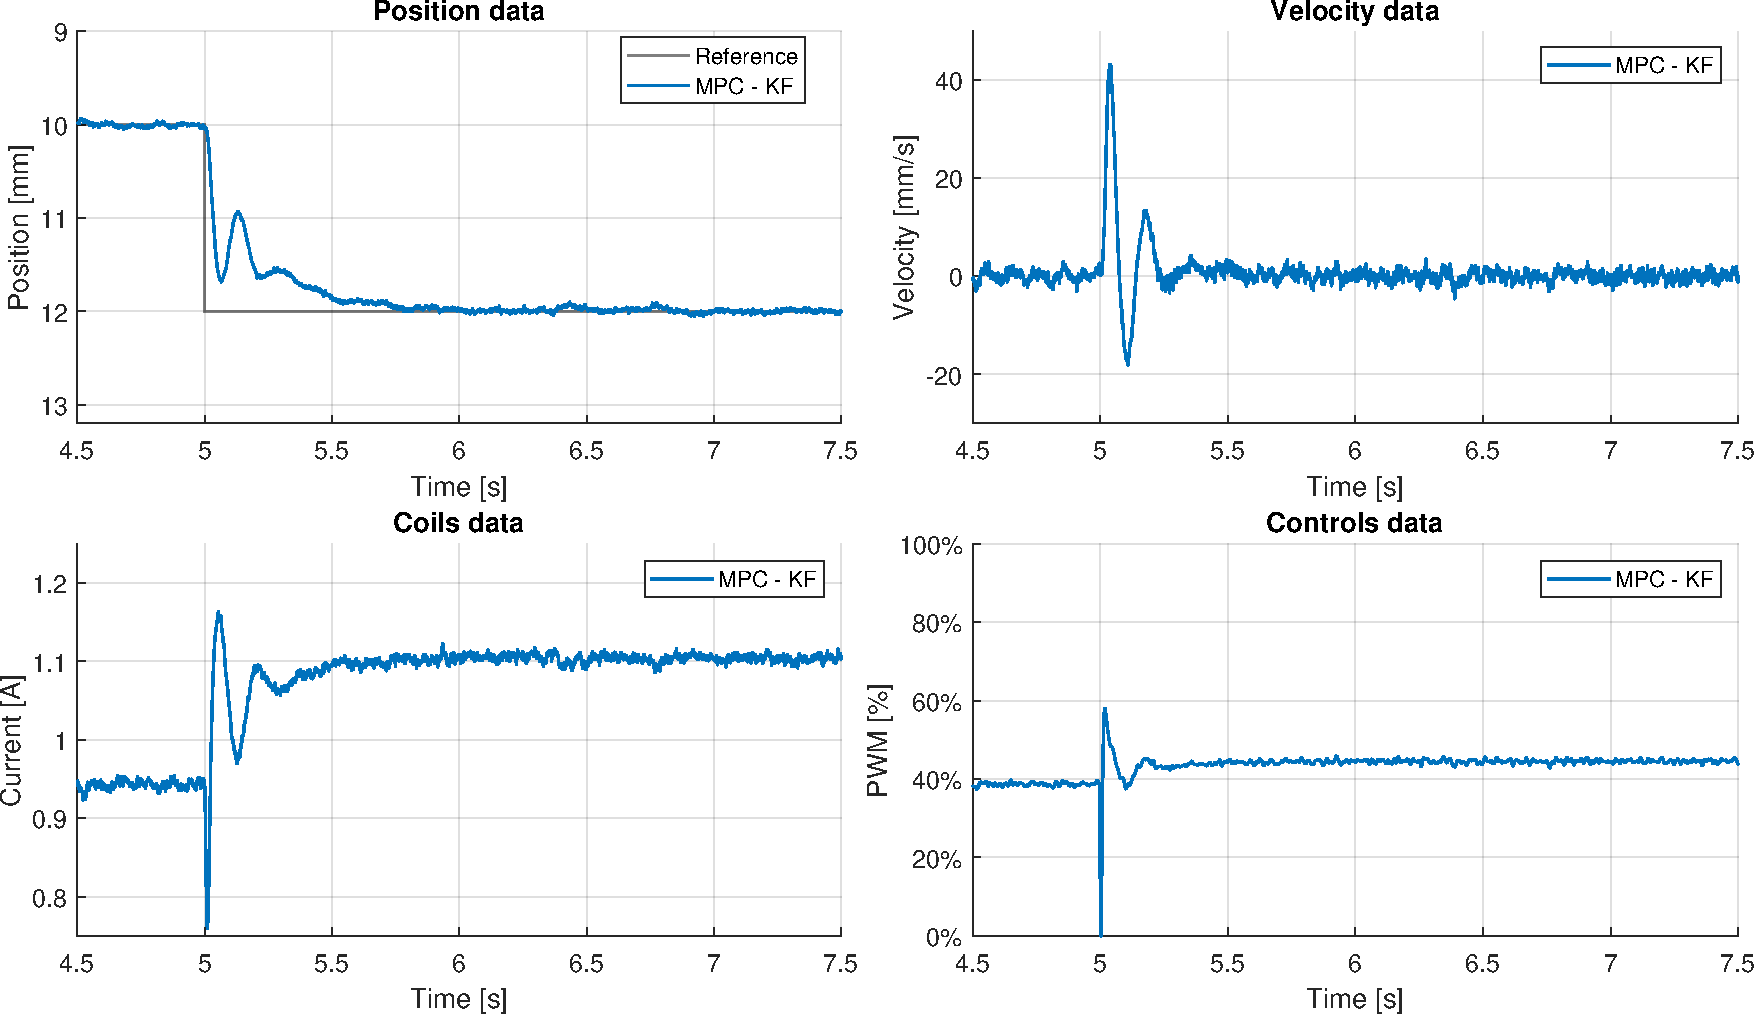
\includegraphics[width=1\linewidth]{./img/MATLAB/results/step_MPC_KF.pdf}
    \caption{Step Response (MPC)}
    \label{fig:step_MPC}
\end{figure}
